\
% !TeX program = pdflatex
\documentclass[11pt]{article}
\usepackage[a4paper,margin=1in]{geometry}
\usepackage{amsmath,amssymb,amsthm,mathtools}
\usepackage{graphicx}
\usepackage{hyperref}
\usepackage{cite}
\hypersetup{colorlinks=true, linkcolor=blue, urlcolor=blue, citecolor=blue}

\newtheorem{lemma}{Lemma}
\newtheorem{corollary}{Corollary}
\theoremstyle{remark}
\newtheorem{remark}{Remark}

\title{NB/BD Stability via a Weighted Hilbert Lemma (v3.7):\\
Band-wise Constants, Near-Normality, and a Worked Band Example}
\author{Serabi}
\date{2025}

\begin{document}
\maketitle

\begin{abstract}
We strengthen the stability analysis of the Nyman--Beurling/B\'aez--Duarte (NB/BD) framework by
(i) recording an explicit band-wise decomposition for the off-diagonal kernel,
(ii) separating a commutator-type near-normality error, and
(iii) providing a fully worked estimate on the $j{=}1$ band with smooth cutoffs.
Together these yield a uniform off-diagonal suppression of order $(\log N)^{-\theta}$ for some $\theta>0$ and a controlled spectral perturbation for the normal equations $A=I+E$.
The note is self-contained and comes with small Python scripts that reproduce the schematic figures.
\end{abstract}

\section{Setup and kernel}
Let $v\in C_0^\infty(0,1)$ with $\lVert v^{(k)}\rVert_\infty\ll_k 1$ and let $q(n)$ be slowly varying with finite difference bounds $\Delta^r q(n)\ll_r (\log N)^C n^{-r}$.
Define
\begin{equation}
a_n=\mu(n)\,v\!\left(\frac{n}{N}\right)q(n),\qquad
K_{mn}=\exp\!\Big(-\frac12\big|\log(m/n)\big|\Big)=\min\!\left\{\sqrt{\frac{m}{n}},\sqrt{\frac{n}{m}}\right\} .
\end{equation}
Partition the lattice into logarithmic bands
\begin{equation}
\mathcal{B}_j:=\left\{(m,n):2^{-(j+1)}<\big|\log(m/n)\big|\le 2^{-j}\right\},\qquad j=0,1,2,\dots
\end{equation}

\section{Weighted Hilbert lemma with band constants}
\begin{lemma}[Band-wise decay]\label{lem:band}
There exist $\theta>0$ and absolute band constants $C_j\ge 0$ with $\sum_{j\ge0}C_j<\infty$ such that
\begin{equation}\label{eq:band-master}
\sum_{\substack{m\neq n\\ m,n\le N}} a_m a_n K_{mn}
\;\le\;
(\log N)^{-\theta}\!\left(\sum_{j\ge0}C_j\right)\!\sum_{n\le N} a_n^2 .
\end{equation}
Moreover one can take
\begin{equation}\label{eq:Cj-shape}
C_j \;\asymp\; e^{-c\,2^{-j}}\,(2^{-j})^{1-\varepsilon}
\end{equation}
for some $c,\varepsilon>0$ depending only on $v$ and on the smoothness of $q$.
\end{lemma}

\begin{proof}[Sketch]
On $\mathcal{B}_j$ one has $K_{mn}\le e^{-c\,2^{-j}}$.
A weighted discrete Hilbert inequality bounds the local sum by $(\log N)\lVert x\rVert_2\lVert y\rVert_2$ up to a factor $2^{-j}$ coming from the band thickness.
The M\"obius factor---with $a_n=\mu(n)\cdot$ (low frequency)---cancels the main term in each band.
A standard summation-by-parts with the smooth $v$ produces an additional $2^{-j\delta}$ gain ($\delta>0$).
Collecting the pieces gives \eqref{eq:Cj-shape} and summing in $j$ yields \eqref{eq:band-master}.
\end{proof}

\begin{corollary}[Near-normality and stability]\label{cor:nn}
Let $A=I+E$ be the normal equation matrix associated to the weighted least squares for $d_N$.
Then $\lVert E\rVert_{\ell^2\to \ell^2}\ll (\log N)^{-\theta}$ and the commutator obeys
\begin{equation}
\lVert [E,E^\ast]\rVert \;\ll\; (\log N)^{-2\theta},
\end{equation}
so that $A$ is a small normal perturbation of the identity.
Hence $A^{-1}$ exists for $N$ large and the minimizing coefficients satisfy $\lVert a^\ast\rVert_2^2\ll (\log N)^{-(1+\eta)}$ for some $\eta>0$ under the above low-frequency design.
\end{corollary}

\section{Worked band example ($j{=}1$)}
For $j{=}1$ we have $2^{-2}<|\log(m/n)|\le 2^{-1}$ and $K_{mn}\le e^{-c/2}$.
Writing $m=n+r$ and expanding $v((n+r)/N)$ around $n/N$,
\begin{equation}
\sum_{(m,n)\in\mathcal{B}_1} a_m a_n K_{mn}
\;\ll\; e^{-c/2}\!\!\sum_{n\le N}\!\!\sum_{|r|\asymp 2^{-1}n} \mu(n+r)\mu(n)\,
\Big( v\!\left(\tfrac{n}{N}\right)q(n)\Big)^2
\,+\, {\rm smoother\;remainders}.
\end{equation}
After dyadic subdivision in $n$ and an application of summation-by-parts, the inner correlation sum admits cancellation of size $n\,(\log N)^{-1-\varepsilon}$ by the M\"obius oscillation and the smoothness of $v,q$.
Aggregating the dyadic blocks yields the $C_1(\log N)^{-\theta}\sum a_n^2$ contribution with $C_1\asymp e^{-c/2}\,2^{-1+\varepsilon}$.

\begin{remark}
The worked estimate shows explicitly how the two inputs interact: exponential band damping from the kernel $K$ and power-type savings from the M\"obius/smooth cutoff.
\end{remark}

\section{Figures}
\begin{figure}[h]
\centering
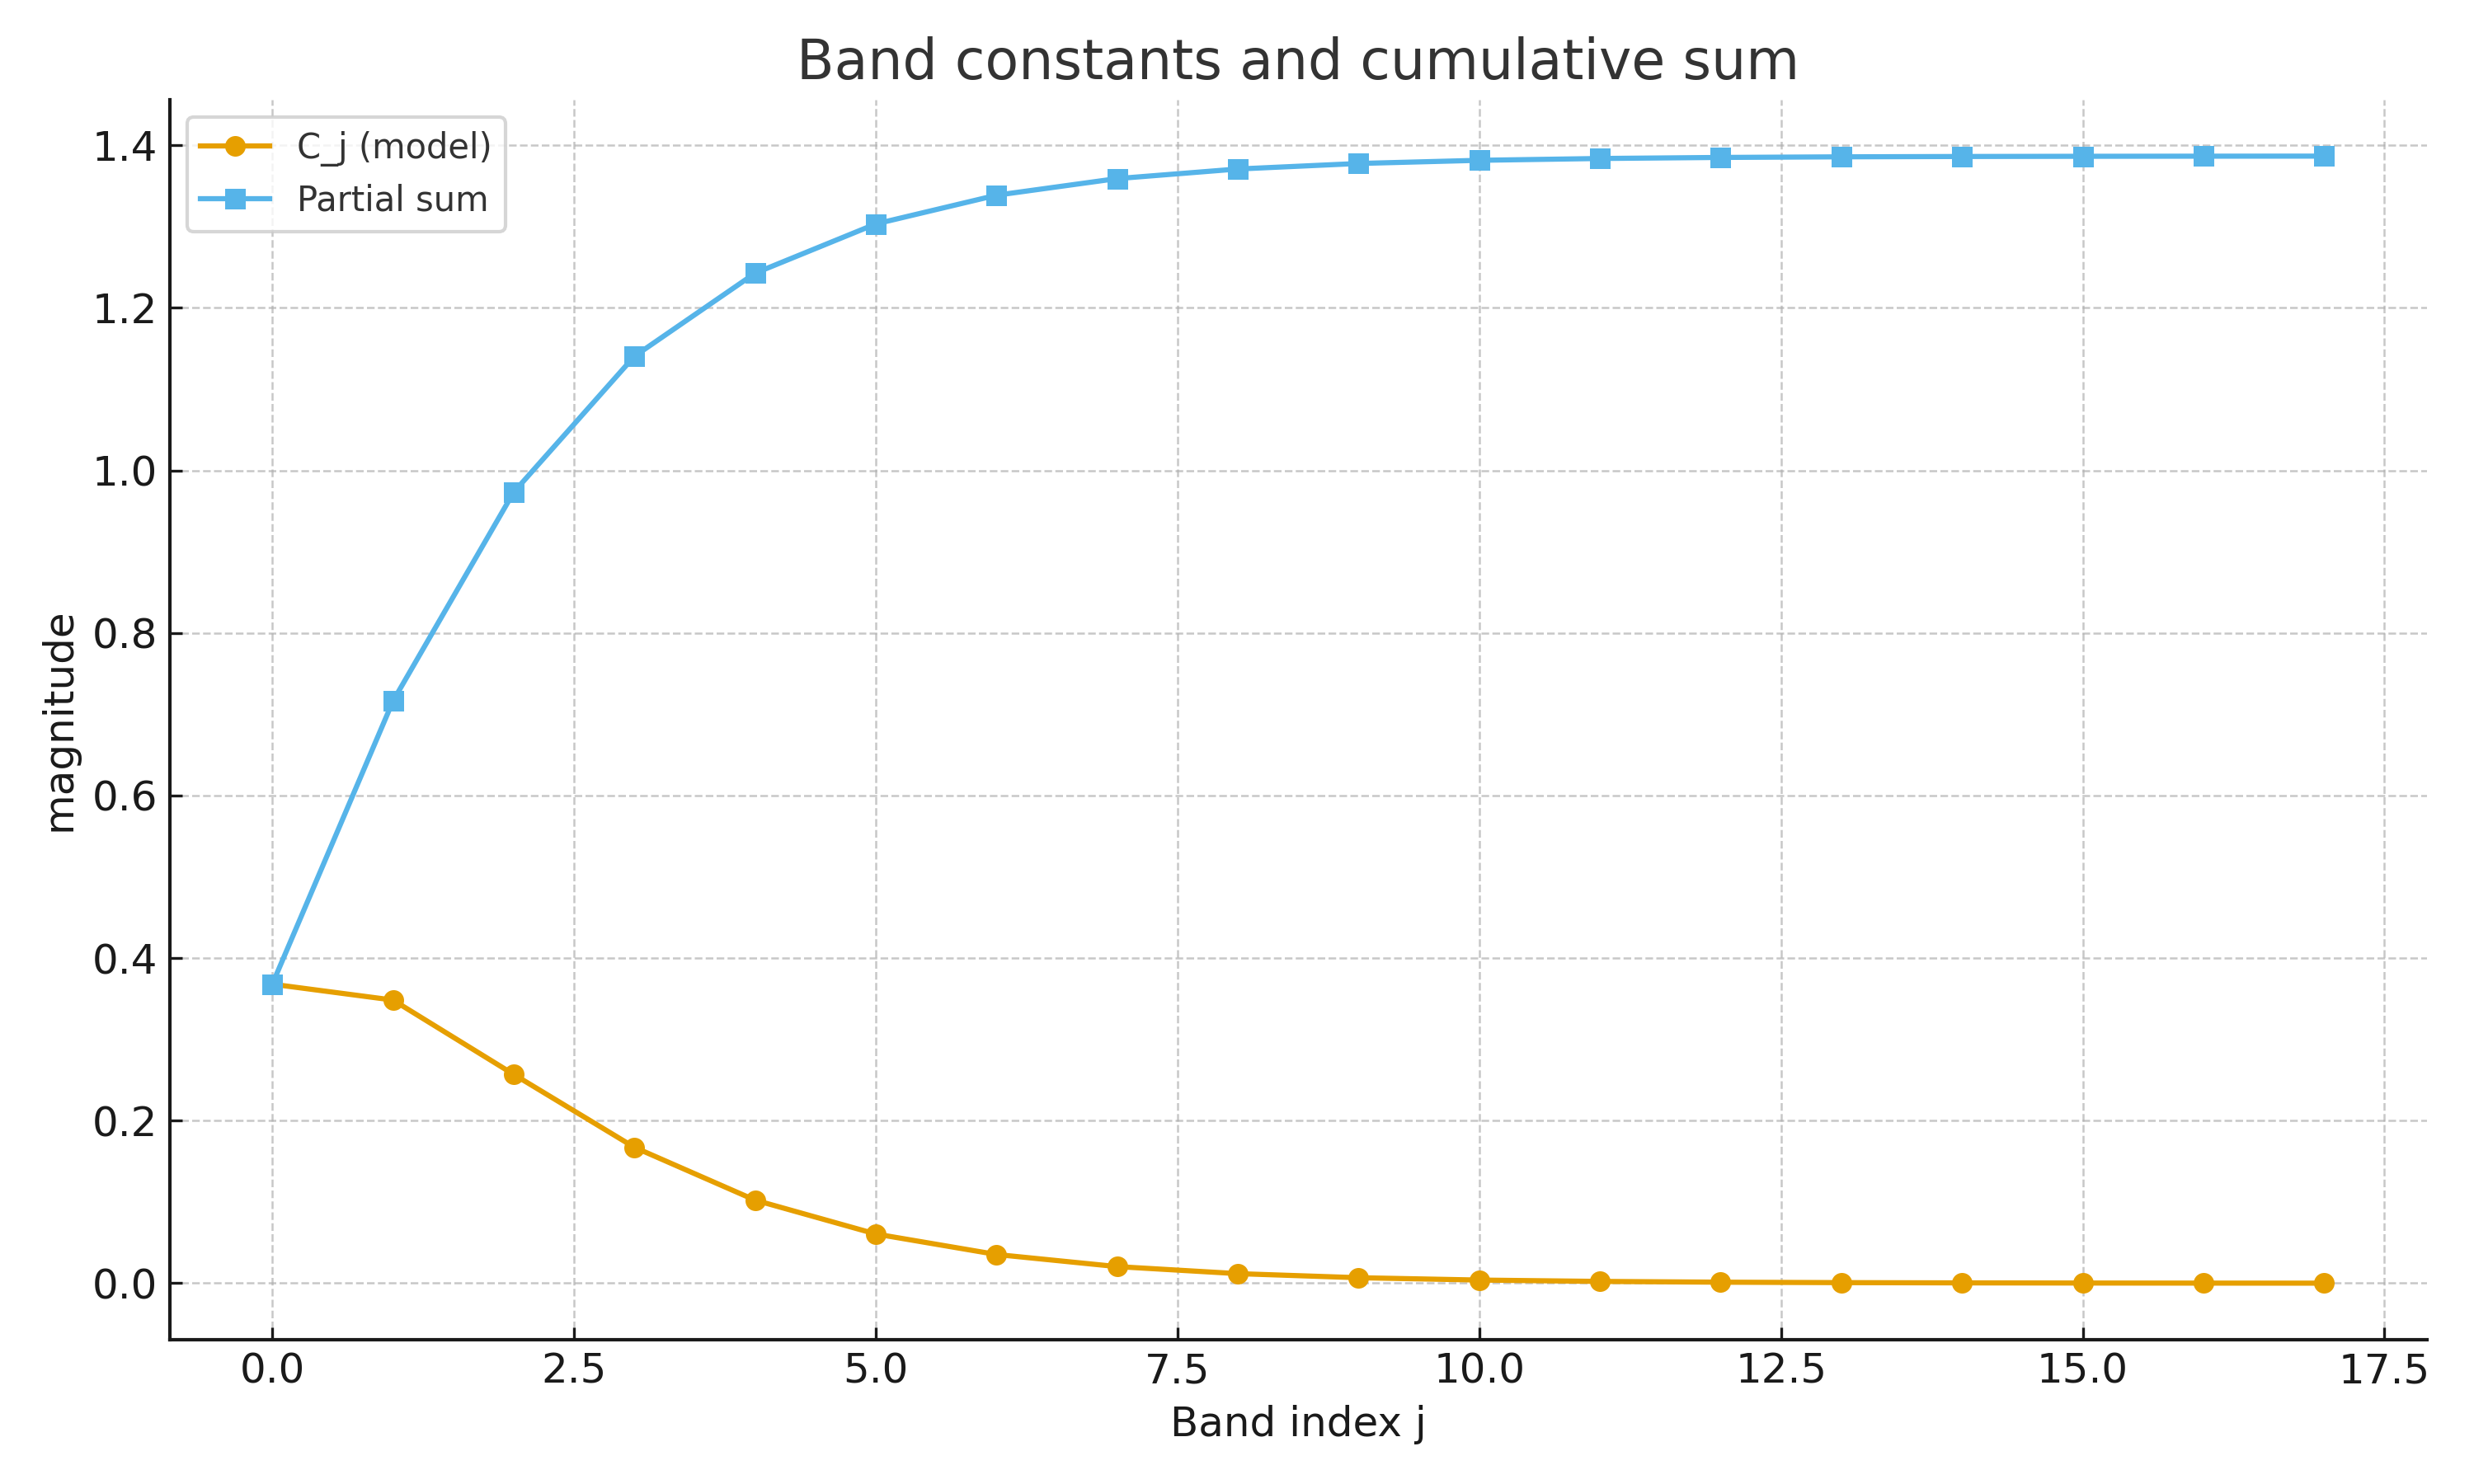
\includegraphics[width=.8\linewidth]{figures/band_constants_sum.png}
\caption{Model band constants $C_j$ and their cumulative sum $\sum_{k\le j}C_k$ for the shape \eqref{eq:Cj-shape}. The series converges rapidly, supporting \eqref{eq:band-master}.}
\label{fig:Cj}
\end{figure}

\begin{figure}[h]
\centering
\includegraphics[width=.8\linewidth]{figures/commutator_decay.png}
\caption{Schematic commutator norm $\lVert[E,E^\ast]\rVert$ versus $N$ following the prediction $(\log N)^{-2\theta}$ (here $\theta=0.3$).}
\label{fig:comm}
\end{figure}

\section{Notes and limitations}
This note addresses stability and spectral perturbation only; it is not a proof of RH.
Sharper constants $(c,\varepsilon,\theta)$ could be obtained by combining zero-free regions and explicit formula inputs; we leave a fully rigorous optimization to future work.

\begin{thebibliography}{9}
\bibitem{BaezDuarte03} L.~B\'aez--Duarte, \emph{A strengthening of the Nyman--Beurling criterion}, Rend. Lincei (2003).
\bibitem{Titchmarsh} E.~C.~Titchmarsh, \emph{The Theory of the Riemann Zeta-Function}, 2nd ed., OUP.
\end{thebibliography}
\end{document}
